\documentclass[../rapport.tex]{subfiles}

\begin{document}

\subsection{Raisonnement initial}
Dans notre code, nous sommes partis du code du \textit{benchmark} qui était mis à disposition, et l'avons adapté à nos besoins. 
Nous avons donc utilisé le \textbf{pipeline} pour pré-process nos données. 
Ce pre-processing inclus toutes les modifications sur les données, avec notamment la gestion des valeurs nulles remplacées selon les stratégies que nous avons choisi. 
Dans notre cas, il a été décidé d'utiliser la stratégie \textbf{mean} pour les \textit{features} numériques, et \textbf{most\_frequent} pour les \textit{features} catégoricielles. 
La stratégie \textbf{mean} permet de remplacer les valeurs manquantes par la valeur moyenne de la colonne dans laquelle elles sont manquantes.
La stratégie \textbf{most\_frequent} permet de remplacer les valeurs manquantes par les catégories les plus présentes dans la colonne.
Ensuite, nous avons fait varier les modèles utilisés dans notre pipeline. 
Lors de nos recherches pour déterminer quels méthodes et modèles nous allions utiliser, nous sommes tombés sur une image de la documentation de \textit{scikit-learn} présentant les algorithmes de recherches à privilégier en fonction des données dont nous disposons. Nous avons donc suivi ce graphique pour déterminer quels seraient les algorithmes intéressants à étudier.

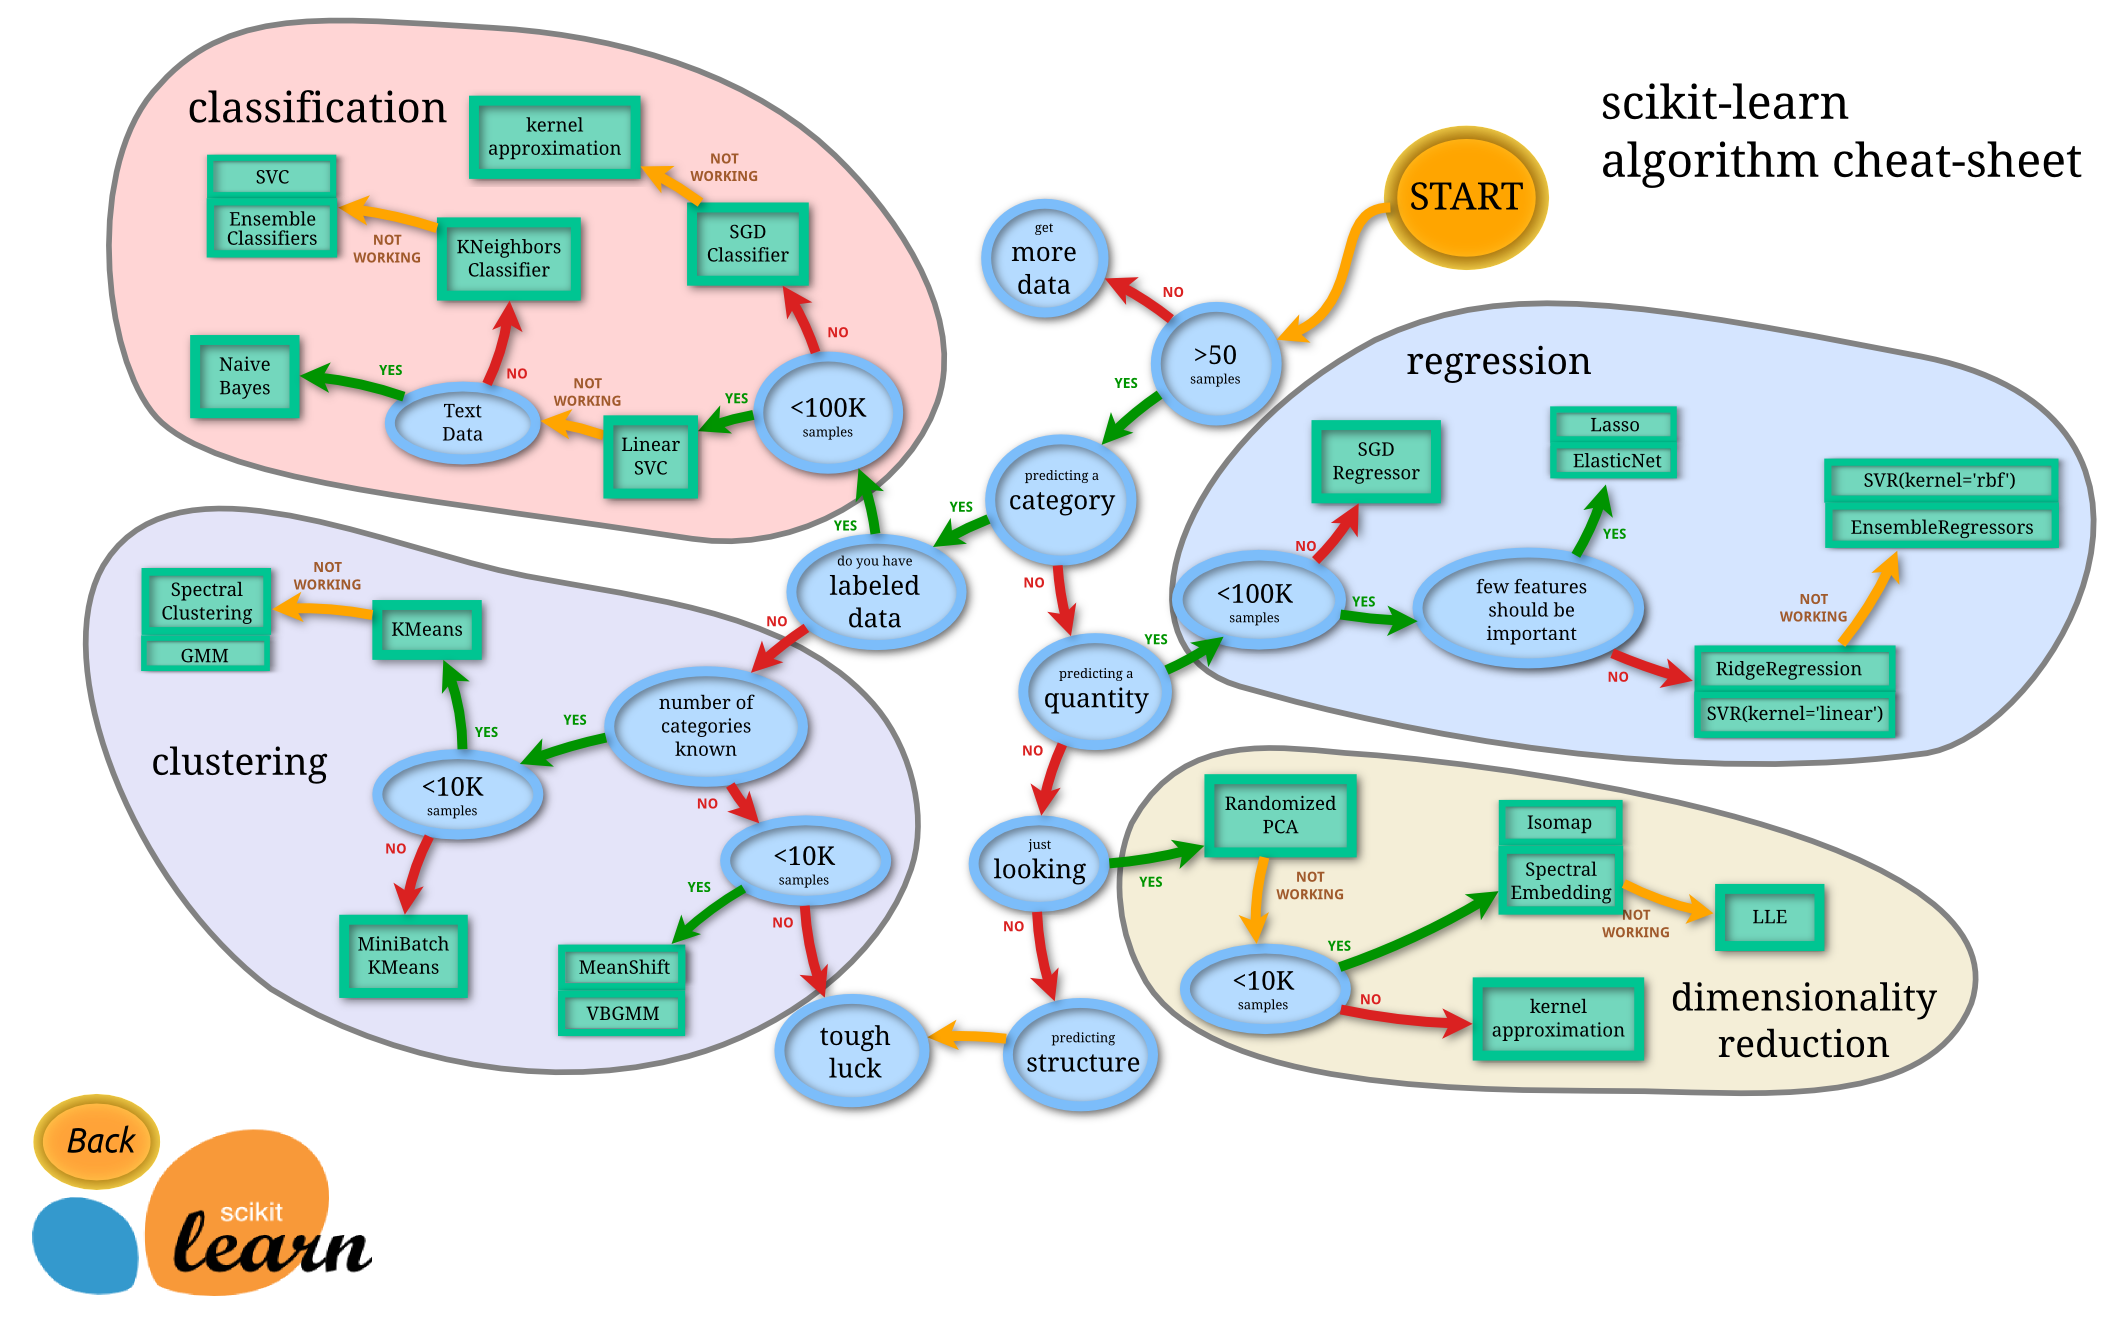
\includegraphics[scale=0.1]{images/ml_map.png}

\subsection{Linear SVC}
En suivant le schéma de la documentation, nous avons donc dans un premier temps cherché à utiliser l'algorithme \textbf{LinearSVC}. 
Cet algorithme est un algorithme qui tente de trouver un hyperplan pour maximiser la distance entre les échantillons classifiés (Définition : documentation scikit-learn).
En essayant d'appliquer cet algorithme à nos données, nous nous sommes aperçu que les résultats n'étaient pas ceux escomptés. 
L'algorithme fonctionne, mais les résultats en sont pas assez intéressants dans notre cas.

\subsection{Logistic Regression}
Après avoir essayé l'algorithme \textbf{LinearSVC}, nous avons essayé l'algorithme \textbf{LogisticRegression}. C'est un algorithme linéaire de classification qui

\subsection{KNN - KNeighborsClassifier}
Le KNN est un algorithme de classification. Celui ci utilise les données d'entrainement pour déterminer la classe d'un nouvel échantillon. Pour cela, il va regarder les K plus proches voisins de l'échantillon et déterminer la classe de l'échantillon en fonction de la classe majoritaire des K plus proches voisins.
\subsection{Random Forest Classifier}
L'algorithme \textbf{RandomForestClassifier} est un algorithme de classification qui utilise un ensemble d'arbres de décisions. L'utilisation de celui ci nous a permis d'augmenter notre score de façon conséquente.
\subsection{Gradient Boosting Classifier}

\subsection{Bagging Classifier}

\subsection{Extra Trees Classifier}
Après avoir essayé les algorithmes précédents, nous avons essayé l'algorithme \textbf{ExtraTreesClassifier}. Cet algorithme nous a permis d'avoir le meilleur score parmi tous les autres. Son fonctionnement est ...
\end{document}
